\chapter{Анализ предметной области}

\section{Общая характеристика предметной области}

Описание предметной области исследования, её особенности и специфика.

\section{Анализ существующих решений}

Обзор существующих решений в исследуемой области.

\begin{figure}[H]
\centering
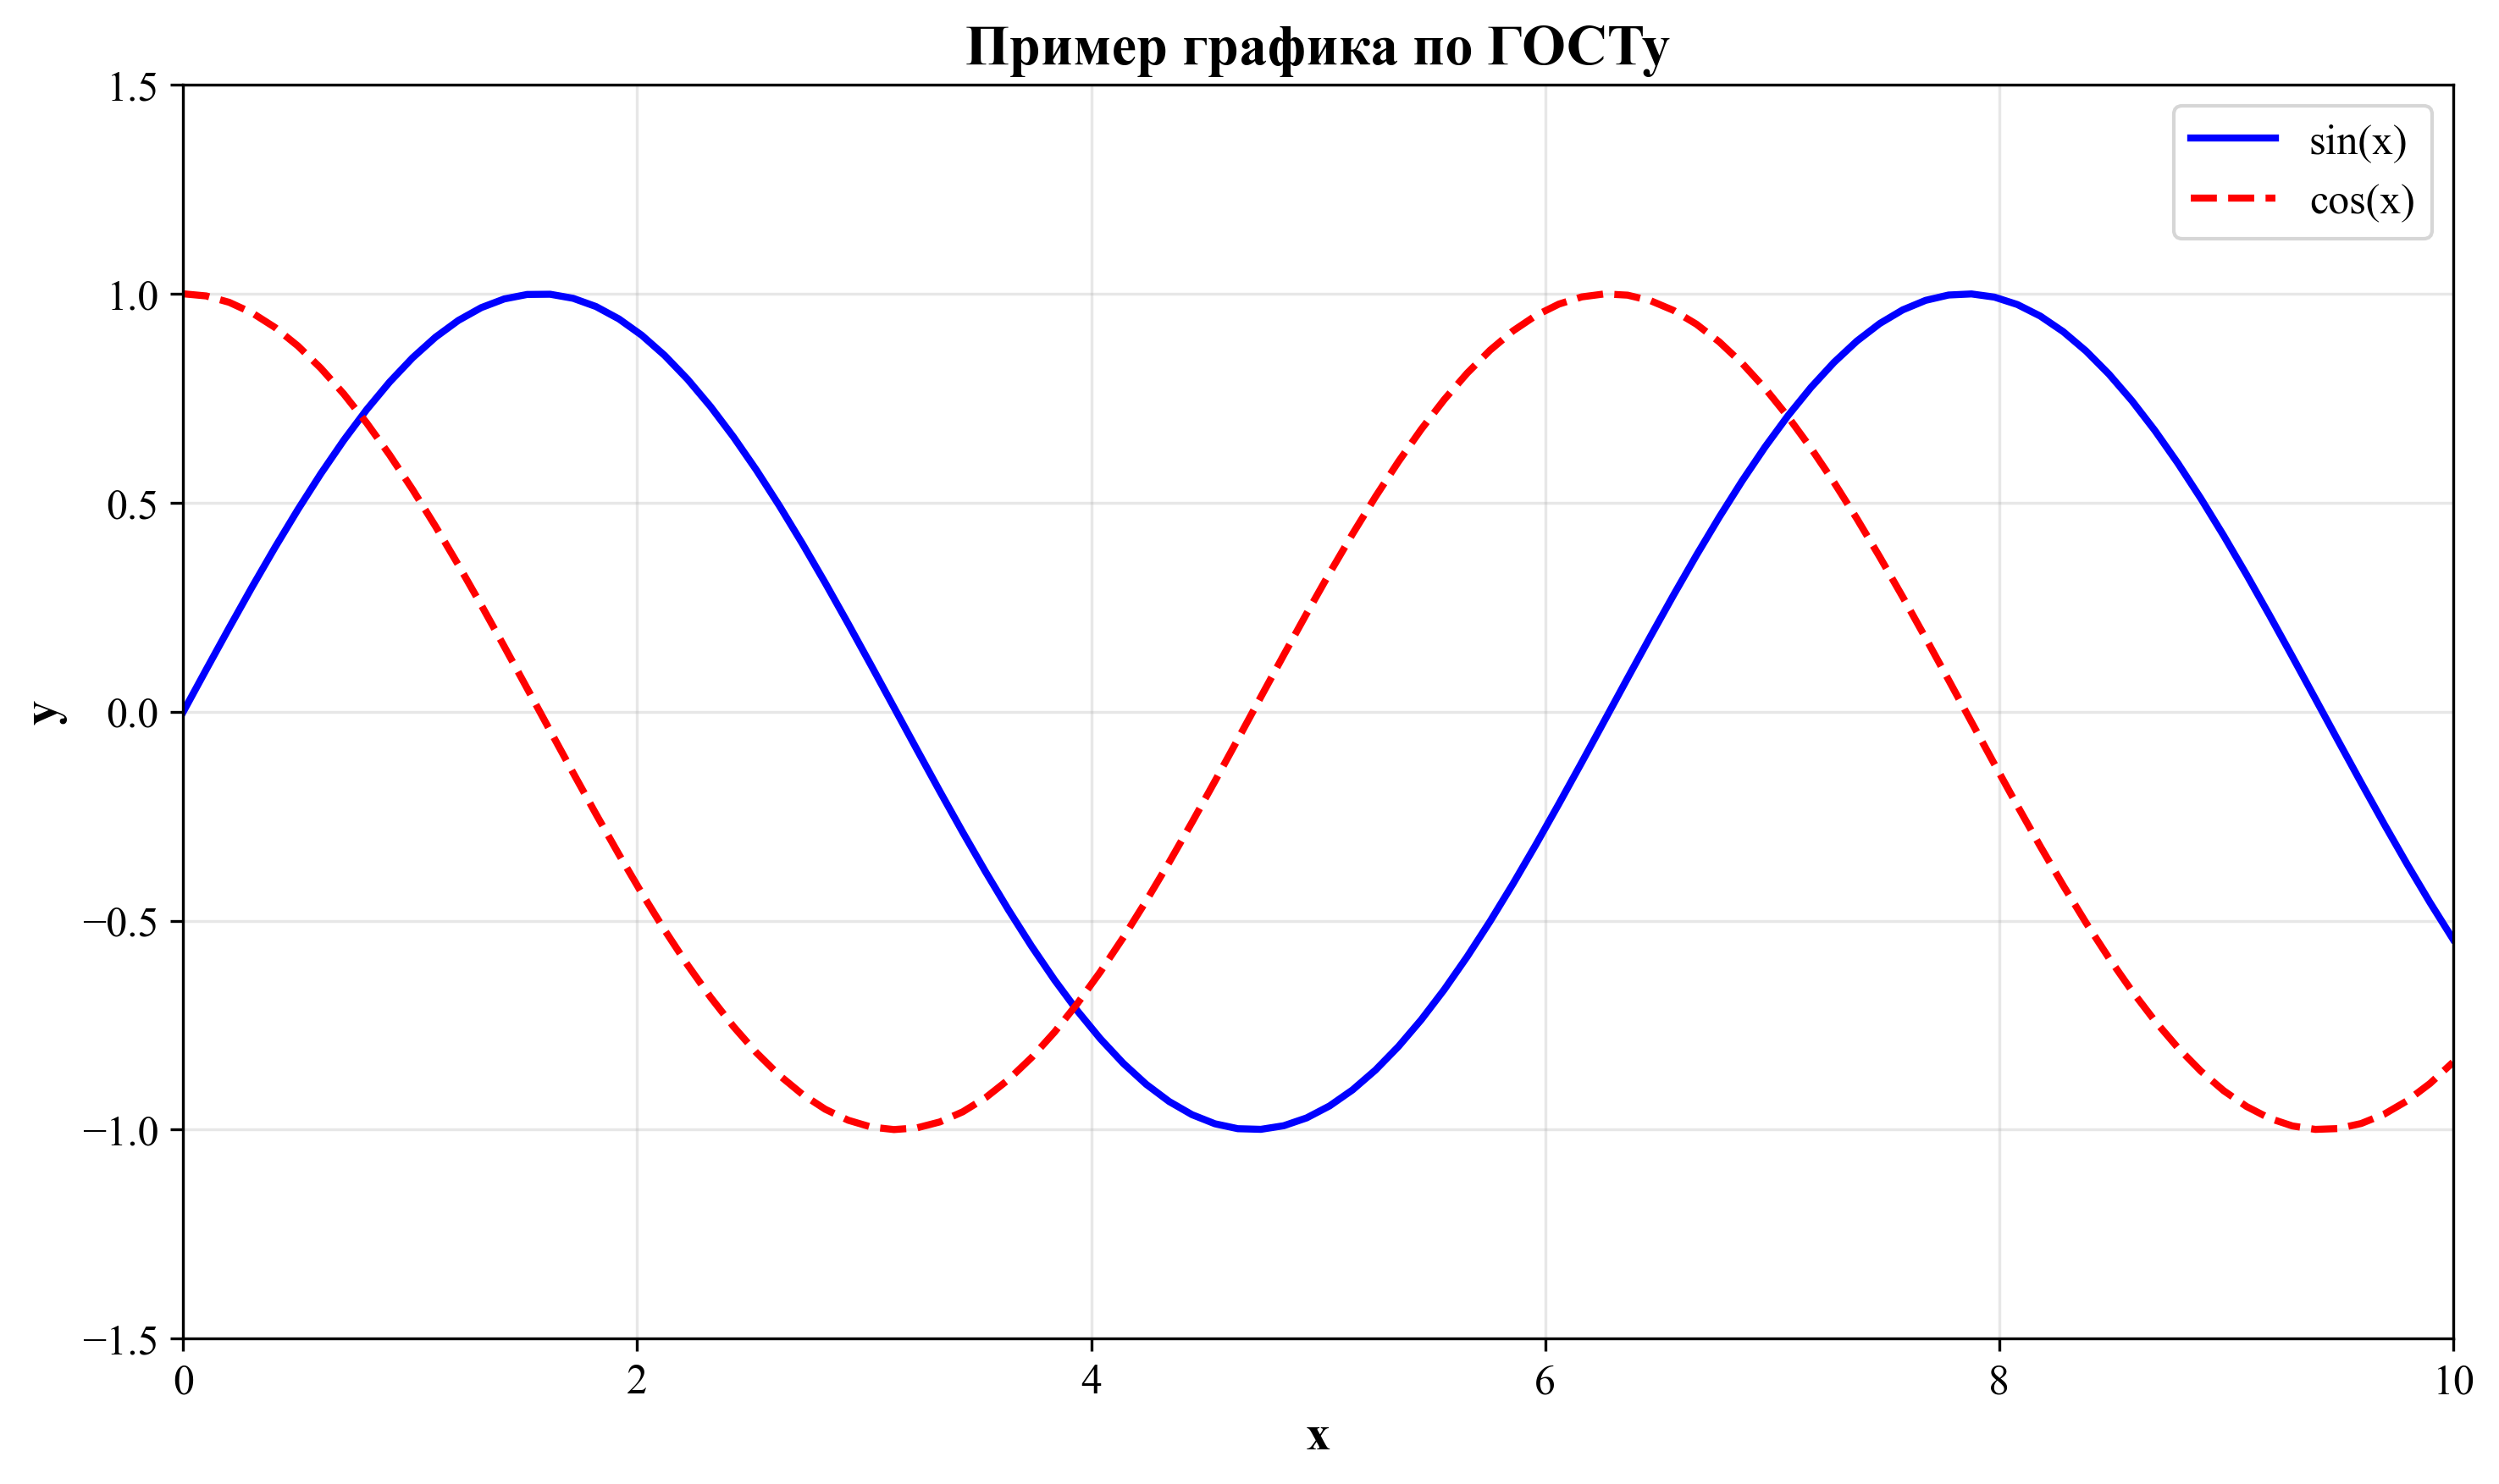
\includegraphics[width=0.6\textwidth]{images/example_plot.png}
\caption{Сравнение производительности алгоритмов}
\label{fig:algorithm_comparison}
\end{figure}

На рисунке \ref{fig:algorithm_comparison} показано сравнение производительности различных алгоритмов обработки данных.

\begin{table}[H]
\centering
\caption{Сравнительный анализ решений}
\label{tab:solutions_comparison}
\begin{tabular}{|l|c|c|c|}
\hline
\textbf{Решение} & \textbf{Скорость} & \textbf{Точность} & \textbf{Стоимость} \\
\hline
Алгоритм A & 95\% & 87\% & 1000 руб. \\
Алгоритм B & 78\% & 92\% & 1500 руб. \\
Алгоритм C & 88\% & 89\% & 800 руб. \\
\hline
\end{tabular}
\end{table}

В таблице \ref{tab:solutions_comparison} представлен сравнительный анализ существующих решений по ключевым параметрам.

\begin{equation}
f(x) = \frac{1}{1 + e^{-x}}
\label{eq:sigmoid}
\end{equation}

Формула \ref{eq:sigmoid} описывает сигмоидную функцию, используемую в машинном обучении.

\begin{CodeBlock}{Python}{Пример реализации алгоритма}{lst:algorithm_implementation}
def sigmoid(x):
    """Calculate sigmoid function"""
    return 1 / (1 + np.exp(-x))

def train_model(X, y, epochs=1000, lr=0.01):
    """Train model"""
    weights = np.random.randn(X.shape[1])
    
    for epoch in range(epochs):
        predictions = sigmoid(X @ weights)
        error = y - predictions
        weights += lr * X.T @ error
    
    return weights
\end{CodeBlock}

В листинге \ref{lst:algorithm_implementation} показана реализация алгоритма обучения модели с использованием сигмоидной функции.

\subsection{Решение 1}

Описание первого решения, его характеристики.

\subsection{Решение 2}

Описание второго решения, его характеристики.

\section{Выявление проблем и недостатков}

Анализ проблем и недостатков существующих решений.

\section{Требования к решению}

Формулирование требований к разрабатываемому решению.

\subsection{Функциональные требования}

Список функциональных требований.

\subsection{Нефункциональные требования}

Список нефункциональных требований.

\section{Выводы по главе}

Краткие выводы по анализу предметной области.
